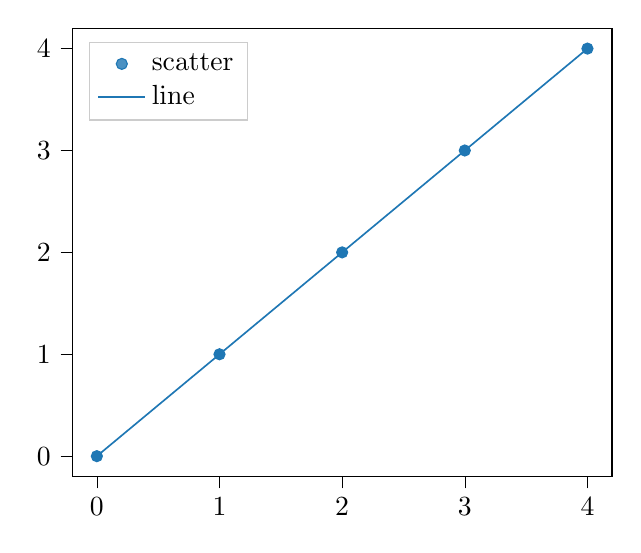
\begin{tikzpicture}

\definecolor{darkgray176}{RGB}{176,176,176}
\definecolor{lightgray204}{RGB}{204,204,204}
\definecolor{steelblue31119180}{RGB}{31,119,180}

\begin{axis}[
legend cell align={left},
legend style={
  fill opacity=0.8,
  draw opacity=1,
  text opacity=1,
  at={(0.03,0.97)},
  anchor=north west,
  draw=lightgray204
},
tick align=outside,
tick pos=left,
x grid style={darkgray176},
xmin=-0.2, xmax=4.2,
xtick style={color=black},
y grid style={darkgray176},
ymin=-0.2, ymax=4.2,
ytick style={color=black}
]
\addplot [draw=steelblue31119180, fill=steelblue31119180, mark=*, only marks]
table{%
x  y
0 0
1 1
2 2
3 3
4 4
};
\addlegendentry{scatter}
\addplot [semithick, steelblue31119180]
table {%
0 0
1 1
2 2
3 3
4 4
};
\addlegendentry{line}
\end{axis}

\end{tikzpicture}
